\chapter{Rigid Body Kinematics and Rotation Matrix}
	
	\de{Kinematic} is the study of purely geometrical aspects of individual positions and motions of rigid bodies, hence cause of motions (forces and torques) are not considered. In particular we define \textbf{bodies} as \textbf{rigid} if for every point $\vett P_1, \vett P_2, \vett P_3$ in it the mutual distance between them and the angle represented by the vector connecting each pair of point are constant (or can be approximated as so):
	\[ \vett P_1 \vett P_2 = \textrm{const.} \qquad \textrm{and} \qquad \angle  \{ \vett P_1 \vett P_2, \vett P_1\vett P_3 \} = \textrm{const.} \hspace{2cm} \forall \vett P_1,\vett P_2, \vett P_3  \textrm{ points} \in \textrm{body} \]
	
\section{Rotation matrix}

	To describe the \de{pose} (\textit{position}) and \de{attitude} (\textit{orientation in space}) of a body respect to another one (or respect to ground) we use the so called \de{reference frame} $\rf{}$ describing the \textbf{configuration} (the set of parameters that fully describes the system) of the body in the space. Considering planar systems, each body has 3 degrees of freedom hence the minimum number of parameters of the configuration is 3; in the spatial case the number increases to 6.
	
	Typically bodies are described in \de{local} (or \textbf{moving}) reference frames $\rfb$ that are obtained as roto-translations of a \de{world} (or \textbf{ground}) reference frame $\rfw$. Given in fact the coordinates $\vett x_b$ of a point $\vett P$ described in the local frame of the body, the absolute position respect to the world frame can be obtained as
	\begin{equation} \label{eq:rot:directtransformation}
		\vett x_w = \vett x_0 + \R \vett x_b
	\end{equation}
	where $\vett x_0$ is the origin of the local frame respect to the world frame (representing so the \textbf{pose}) and $\R$ is a \de{rotation matrix} that describes the \textbf{attitude} of the body in ground coordinates.
	
	\paragraph{Rotation matrix} The rotation matrix, as stated, represent the attitude of a body respect to a given absolute reference. In order to specify such \textit{angular orientation} what we need to do is to describe the vectorial base $\base^b$ of the body in terms of the ground vectorial base $\base^w$ as
	\begin{equation}
		\base^b = \R \base^w
	\end{equation}
	In particular the nine elements of the matrix $\R$ are the generalized coordinates that describes the angular orientation of the body in the base $\base^w$. In particular if we consider that the 3 versor that generates the base $\bb$ expressed in the world frame are $\vers i_b = (i_{b,x}, i_{b,y}, i_{b,z})$, $\vers j_b = (j_{b,x}, j_{b,y}, j_{b,z})$, $\vers k_b = (k_{b,x}, k_{b,y}, k_{b,z})$ then the matrix $\R$ can be regarded as
	\begin{equation} \label{eq:rot:rotationmatrix}
		\R= \matrix{\vers i_b & \vers j_b & \vers k_b} = \matrix{ i_{b,x} & j_{b,x} & k_{b,x} \\ 
		i_{b,y} & j_{b,y} & k_{b,y} \\
		i_{b,z} & j_{b,z} & k_{b,z} \\} \quad \textrm{or alternatively} \quad \matrix{ u_x  &  v_x & w_x \\ u_y  &  v_y & w_y \\ u_z  &  v_z & w_z }
	\end{equation}	
	An important aspect to keep in mind is that a base, to be so, must have that the scalar product between any different versor is zero and between the same direction must be unitary, mathematically
	\[ \vers e_i \cdot \vers e_j = \delta_{ij} = \begin{cases}
		1 \qquad & i = j \\ 0 & i \neq j
	\end{cases} \]
	This means that the rotation matrix $\R$, in order to be a proper base, must withstand the following six constraints described by all the possible combination $i,j$:
	\begin{equation} \label{eq:rot:constraints}
		\sum_{k=1}^3 r_{ik} r_{jk} = \delta_{ik} \hspace{2cm} i,j \in \{1,2,3\}
	\end{equation}
	A base is also characterized by being \textit{right-handed} (the order of the versor can be described using the \textit{right hand rule}) and mathematically this means imposing $\vers e_1 \cdot( \vers e_2\times \vers e_3) = 1$. Overall the rotation matrix $\vett R$ has \textbf{9 generalized coordinates} (elements of the matrix), but only \textbf{3} of them are \textbf{independent} because we have \textbf{6 constraints} determined by equation \ref{eq:rot:constraints}. This intuitively proves the fact that in order to describe the \textit{orientation} of a rigid body in space only 3 parameters are required.
	
	As it will be shown different (and more practical ways) to represent such rotation matrix will be present in order to have just 3 parameters (and not 9 subjected to 6 constraints, increasing the complexity of the problem).
	
	Another important property related to the rotation matrix $\R$ is that it belongs to the \de{special orthogonal matrices} $SO(N)$ of order $N$ (and in our case of spatial kinematic we have $N=3$) that's characterized by having the inverse of $\R$ equals to it's transposed; we in fact have tat
	\begin{equation}
		\Rinv \R= \R^T \R= \R \R^T = \I \hspace{1cm} \Leftrightarrow \hspace{1cm} \Rinv = \R^T
	\end{equation}
	By this means equation \ref{eq:rot:directtransformation} can be inverted in order to express the coordinates $\vett x_b$ of a point in the body reference frame as function of the ground coordinates $\vett x_w$ as 
	\begin{equation} \label{eq:rot:inversetransformation}
		\vett x_b = \Rinv \big(\vett x_w - \vett x_0\big) = \R^T \vett x_w - \R^T \vett x_0
	\end{equation}

	\subsection{Transformation matrix}	
		
		The \de{transformation matrix} $\rf{}$ is a $4\times 4$ matrix that's used to fully describe the roto-translation transformation that has to be applied in order to determine the world coordinates $\vett x_w = (x_w,y_w,z_w)$ of a point knowing it's \textit{position} in the local frame $\vett x_b = (x_b,y_b,z_b)$, it's pose $\vett o^w = (x_0,y_0,z_0)$ and orientation $\R$ respect to the global frame:
		\begin{equation}
				\ref{eq:rot:directtransformation}  \mapsto \vector{x_w \\ y_w \\ z_w \\ 1} = \matrix{ \begin{array}{c c c | c}
						&&& x_0 \\
						&\R&& y_0 \\
						&&& z_0 \\ \hline
						0&0&0&1
				\end{array}} \vector{x_b \\ y_b \\ z_b \\ 1} 			
		\end{equation}
		We can see that this construction directly determines the direct transformation described in equation \ref{eq:rot:directtransformation}, but we can also determine the transformation matrix of the inverse transformation as
		\begin{equation}
				\ref{eq:rot:inversetransformation}  \mapsto \vector{x_b \\ y_b \\ z_b \\ 1} = \matrix{ \begin{array}{c c c | c}
						&&& \\
						&\R^{-1}&& -\Rinv \vett o^w \\
						&&& \\ \hline
						0&0&0&1
				\end{array}} \vector{x_w \\ y_w \\ z_w\\ 1}
		\end{equation}
		
		\paragraph{Reference frames as sequence of  transformations} Given a world reference frame $\rfw$ that's hence fixed, local frames associated to bodies are described in such immovable space using a combination of roto-translations. Given for example two transformation $\rf 1,\rf 2$ the order on which we perform the transformations heavily affects the final frame, and in general
		\[ \rf 1 \rf 2 \neq \rf 2\rf 1 \]
	
		\paragraph{Pure translation} If we consider a reference frame $\rf 2$ defined as pure translation of a frame $\rf 1$ (that's also a pure translation of a world reference frame $\rfw$), as shown in figure \ref{fig:rot:translation}, defined by the transformation matrices 
		\[ \rf 1 = \transformationmatrix{ &&& x_{01}^w \\ & \I&& y_{01}^w \\ &&& z_{01}^w \\ \hline 0 & 0 & 0 & 1 } \hspace{2cm} \rf 2 = \transformationmatrix{ &&& x_{02}' \\ & \I&& y_{02}' \\ &&& z_{02}' \\ \hline 0 & 0 & 0 & 1 } \]
		in order to describe the second reference frame into global coordinate system we have to perform the operation $\rf 1 \rf 2$. Performing algebraically the operation we indeed retrieve the intuitive result of a transformation matrix $\rf 2^w$ with no rotation ($\rot = \I$) and center of the base in  $\vett x_1^w + \vett x_2'$, in fact
		\[ \rf 2^w = \rf 1\rf 2 = \transformationmatrix{ &&& x_{01}^2 + x_{02}' \\ & \I&& y_{01}^2 + y_{02}' \\ &&& z_{01}^2 + z_{02}' \\ \hline 0 & 0 & 0 & 1 } \]
		
		\begin{SCfigure}[2][bht]
			\centering 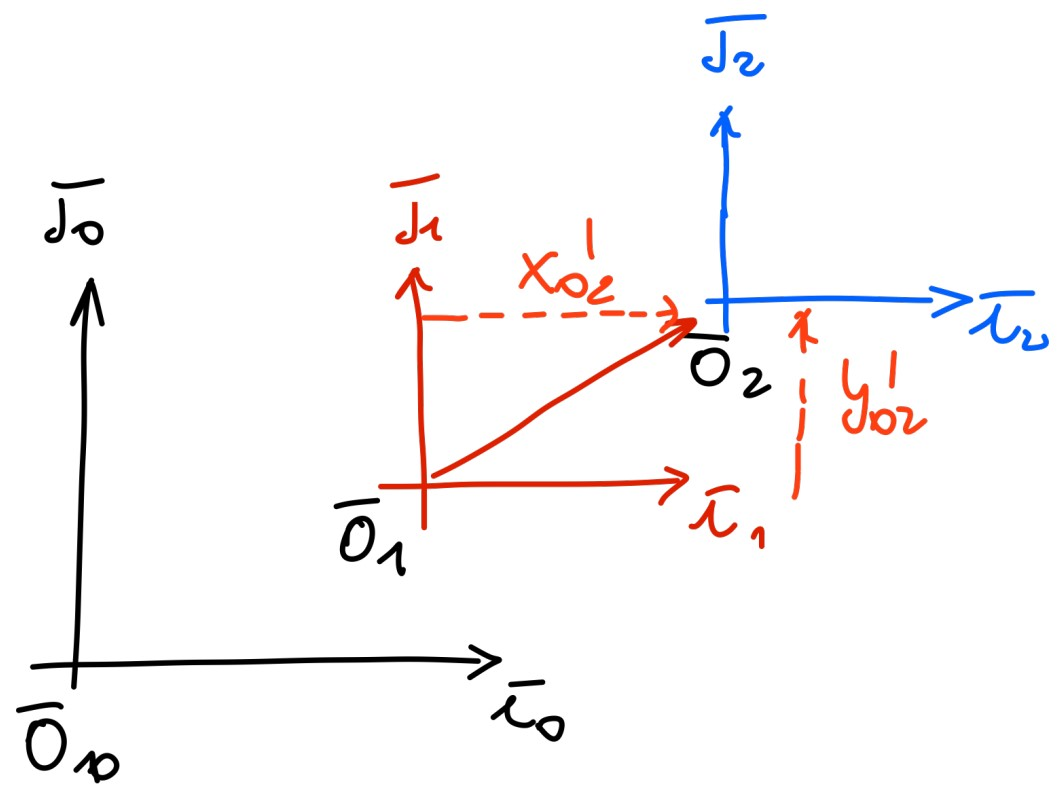
\includegraphics[width=5cm]{translationframe}
			\caption{multiple transformations of pure translation; in this case, for sake of simplicity, the planar case has been considered.} \label{fig:rot:translation}
		\end{SCfigure}
		
		\paragraph{Pure rotation} Considering a reference frame $\rf 2$ that a pure rotation (along the $z$ axis) of an angle $\beta$ respect to a reference frame $\rf 1$ characterized by a pure rotation of angle $\alpha$ respect to the reference frame $\rfw$ (figure \ref{fig:rot:rotational}), their transformation matrices are
		\[ \rf 1 = \transformationmatrix{\cos \alpha & -\sin \alpha & 0 & 0 \\ \sin\alpha & \cos \alpha & 0 & 0 \\ 0 & 0 & 1 & 0 \\ \hline 0 & 0 & 0 & 1} \hspace{2cm} \rf 2 = \transformationmatrix{\cos \beta & -\sin \beta & 0 & 0 \\ \sin\beta & \cos \beta & 0 & 0 \\ 0 & 0 & 1 & 0 \\ \hline 0 & 0 & 0 & 1} \]
		In order to determine the transformation of the second reference frame respect to the ground we so have to compute the product $\rf 1 \rf 2$ between the transformation matrix, hence
		\[ \rf 2^w = \rf 1 \rf 2 = \transformationmatrix{\cos \alpha \cos \beta -\sin\alpha\sin\beta & -\cos \alpha \sin \beta -\sin\alpha \cos \beta & 0 & 0 \\ \sin\alpha\cos\beta + \cos\alpha\sin\beta & -\sin\alpha\sin\beta + \cos\alpha\cos\beta & 0 & 0 \\ 0 & 0 & 1 & 0 \\ \hline 0 & 0 & 0 & 1} \]
		Using so Prostaferesi's equation involving the sum of the argument in (co)sine functions we obtain the intuitive result of a pure revolution of $\alpha + \beta$ along the $z$ axis:
		\[ \rf 2^w = \transformationmatrix{\cos (\alpha +\beta) & -\sin (\alpha + \beta) & 0 & 0 \\ \sin(\alpha + \beta) & \cos (\alpha + \beta) & 0 & 0 \\ 0 & 0 & 1 & 0 \\ \hline 0 & 0 & 0 & 1} \]
		\begin{SCfigure}[2][bht]
			\centering 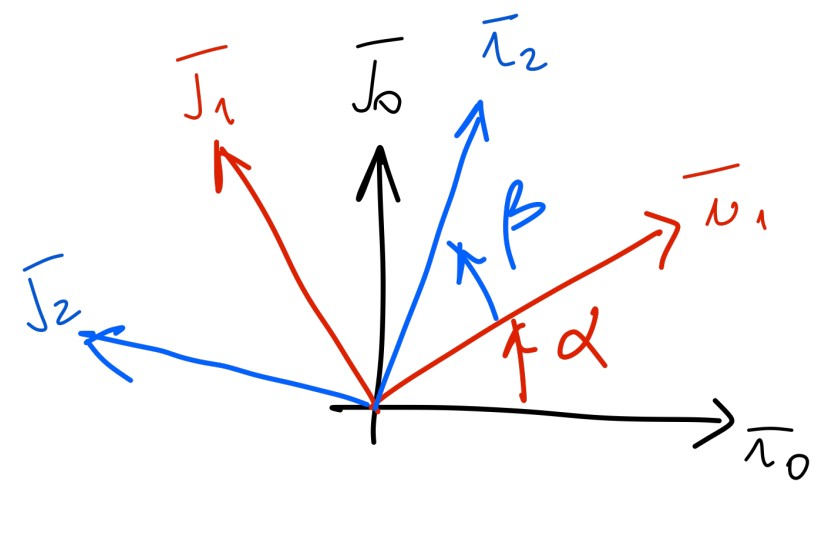
\includegraphics[width=5cm]{rotational}
			\caption{multiple transformations of pure rotation revolving the $z$ axis.} \label{fig:rot:rotational}
		\end{SCfigure}
		
		\paragraph{Rotation and translation} In the case of pure rotation/translation the reference frame that we have obtained was the same if we would have applied the transformation in reversed order, however this are only particular case. If we consider a translation $\rf 1$ and a rotation $\rf 2$ defined by matrices
		\[  \rf 1 = \transformationmatrix{ &&& x_{01}^w \\ & \I&& y_{01}^w \\ &&& 0 \\ \hline 0 & 0 & 0 & 1 }  \hspace{2cm} \rf 2 = \transformationmatrix{\cos \alpha & -\sin \alpha & 0 & 0 \\ \sin\alpha & \cos \alpha & 0 & 0 \\ 0 & 0 & 1 & 0 \\ \hline 0 & 0 & 0 & 1} \]
		Intuitively the reference frame obtain by firstly applying the translation ($\rf 1$) is different from the one obtained by rotating first ($\rf 2$), as also shown in figure \ref{fig:rot:transforder}, in fact by performing the matrix calculations we obtain
		\[ \rf 1 \rf 2 = \transformationmatrix{ &&& x_{01}^w \\ &\rot_\alpha && y_{01}^w \\ &&& 0 \\ \hline 0&0&0& 1} \hspace{1.5cm} \rf 2 \rf 1  = \transformationmatrix{ &&& x_{01}^w \cos\alpha  - y_{01}^2 \sin\alpha \\ &\rot_\alpha && x_{01}^2 \sin\alpha + y_{01}^w \cos\alpha \\ &&& 0 \\ \hline 0&0&0& 1}  \]
		
		\begin{figure}[bht]
			\centering 
			\begin{subfigure}{0.48\linewidth}
				\centering 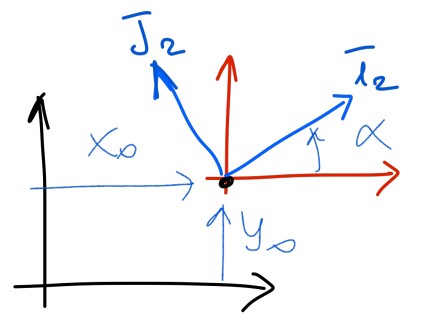
\includegraphics[width=5cm]{rototrans-1} \caption{}
			\end{subfigure}
			\begin{subfigure}{0.48\linewidth}
				\centering 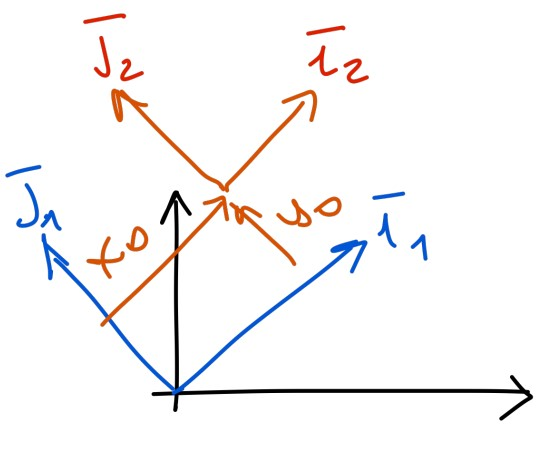
\includegraphics[width=5cm]{rototrans-2} \caption{}
			\end{subfigure}
			\caption{reference frame obtained by first translating and than rotating $(a)$ and first rotating and then translating $(b)$.} \label{fig:rot:transforder}
		\end{figure}
	
	\subsection{Primitive rotation matrices and sequences of rotations}	
		
		\begin{figure}[bt]
			\centering 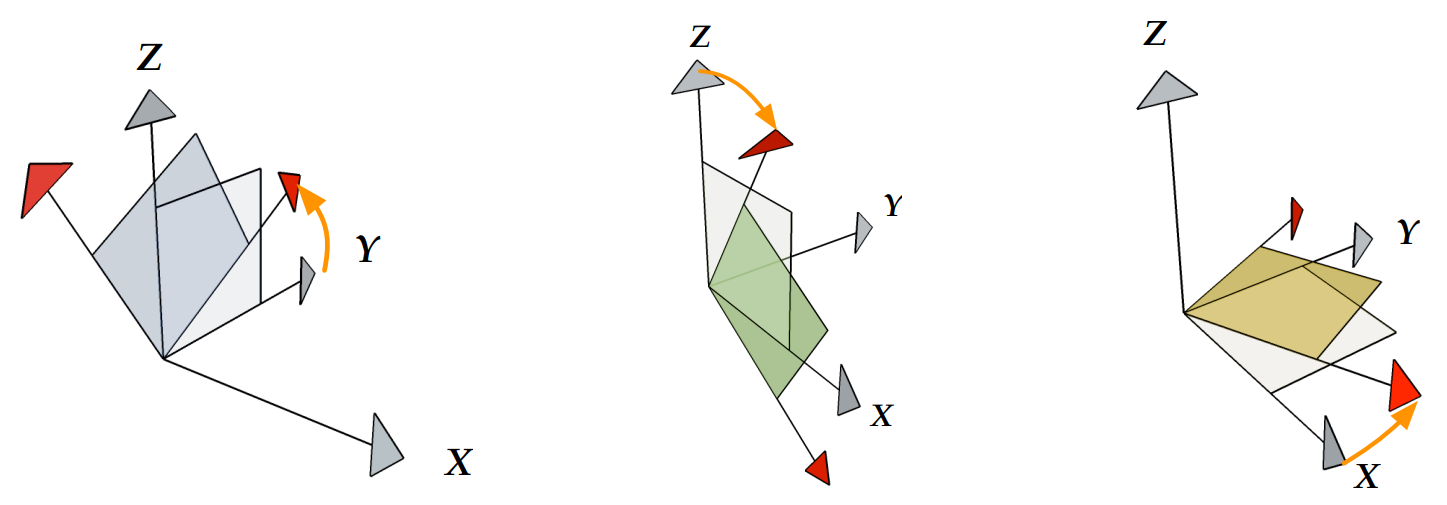
\includegraphics[width=10cm]{rotationmatrices}
			\caption{rotation matrices respect to the $x$ (left), $y$ (middle) and $z$ (right) axis.}
		\end{figure}
	
		As stated previously, the rotation matrix $\R$ (equation \ref{eq:rot:rotationmatrix}) contains 9 parameters 3 of which are independent (the other 6 are constrained by the conditions on the mutual orthogonality) and so a \textit{easier} formulation can be achieved using only 3 parameters. In this sense the angular orientation of the vectorial base $\bb$ can be though as the result of 3 successive rotation along axis; considering as example the sequence
		\[  \bb = \underbrace{\R_1(\theta) \R_2(\phi) \R_3(\psi) }_\R \bw \qquad \leftrightarrow \qquad \bb = \R_x(\theta) \R_y(\phi) \R_z(\psi) \bw \]
		a local frame can be obtained by firstly rotating the global frame along the third ($z$) axis by an angle $\psi$. This operation determines a local frame ${\bb}''$ on top of which a second rotation of angle $\phi$ along the second ($y$) axis is performed. That generates another vectorial space ${\bb}'$ that finally determines the local base $\bb$ as a rotation of an angle $\theta$ along the first ($x$) axis.
		
		In particular the \textbf{primitive rotation matrices} are expressed as
		\begin{equation}
			\R_x(\theta) = \matrix{ 1 & 0 & 0 \\ 0 & \cos\theta &-\sin\theta \\ 0 & \sin\theta &\cos\theta } \quad 
			\R_y(\theta) = \matrix{ \cos\theta & 0 & \sin\theta \\ 0 & 1 & 0 \\ -\sin\theta & 0 & \cos\theta } \quad 
			\R_z(\theta) = \matrix{ \cos\theta & - \sin\theta & 0 \\ \sin\theta & \cos\theta & 0 \\ 0 & 0 & 1 } 
		\end{equation}
		
		\paragraph{Euler angles} The \de{Euler angles} are a common choice in the description of the orientation in a body in space and is obtained by the sequence $z(\psi)\rightarrow x(\theta) \rightarrow z(\phi)$ (or \textit{in numbers} by $3\rightarrow 1 \rightarrow 3$) resulting in the transformation
		\begin{equation} \label{eq:kin:eulerangles}
				\R_z(\phi) \R_x(\theta) \R_z(\psi) \  { \footnotesize = \matrix{ 
				\cos \psi\cos\phi - \sin\psi\cos\theta\sin\phi & \sin\psi \cos\theta + \cos\psi \cos\theta\sin\phi & \sin\theta \sin \phi \\
				-\cos\psi\sin\phi - \sin\psi\cos\theta\cos\phi & - \sin\psi\sin\phi + \cos\psi\cos\theta\cos\phi & \sin\theta\cos\phi \\
				\sin\psi \sin\theta& -\cos\psi \sin\theta & \cos\theta} }	
		\end{equation}
		
		\begin{SCfigure}[2][bht]
			\centering 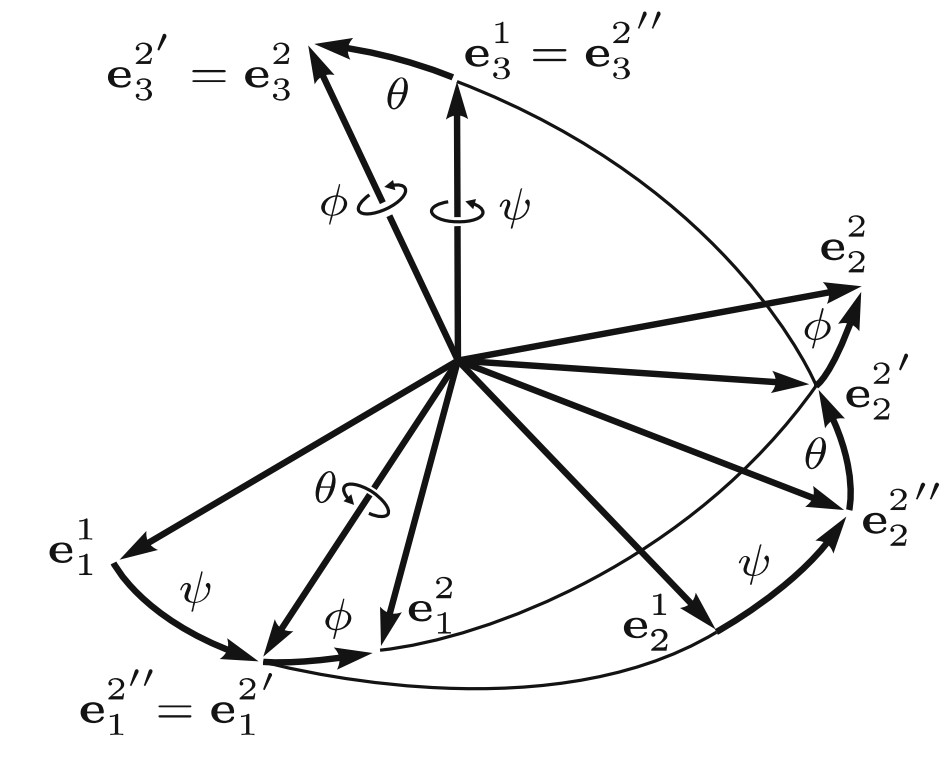
\includegraphics[width=5cm]{eulerangles}
			\caption{representation of the Euler angles $\psi,\theta,\phi$ for representing the attitude of a body.}
		\end{SCfigure}
		
		\paragraph{Bryan angles} \de{Bryan} (or \textbf{Cardan}) \textbf{angles} are associated to another sequence of relative rotations carried along the sequence $1\rightarrow 2 \rightarrow 3$ ($x,y,z$) resulting in
		\begin{equation} 
			 \R_z(\phi_3) \R_y(\phi_2) \R_x(\phi_1) \ { \footnotesize = \matrix{ \cos\phi_2\cos\phi_3 & \cos\phi_1\sin\phi_3 + \sin\phi_1\sin\phi_2\cos\phi_3 & \sin\phi_1\sin\phi_3 - \cos\phi_1\sin\phi_2\cos\phi_3 \\
					-\cos\phi_2\sin\phi_3 & \cos\phi_1 \cos\phi_3 - \sin\phi_1 \sin\phi_2 \sin\phi_3 & \sin\phi_1\cos\phi_3 + \cos\phi_1\sin\phi_2\sin\phi_3 \\
					\sin\phi_2 & -\sin\phi_1\cos\phi_2 & \cos\phi_1\cos\phi_2 } }
		\end{equation}
	
		\begin{SCfigure}[2][bht]
			\centering 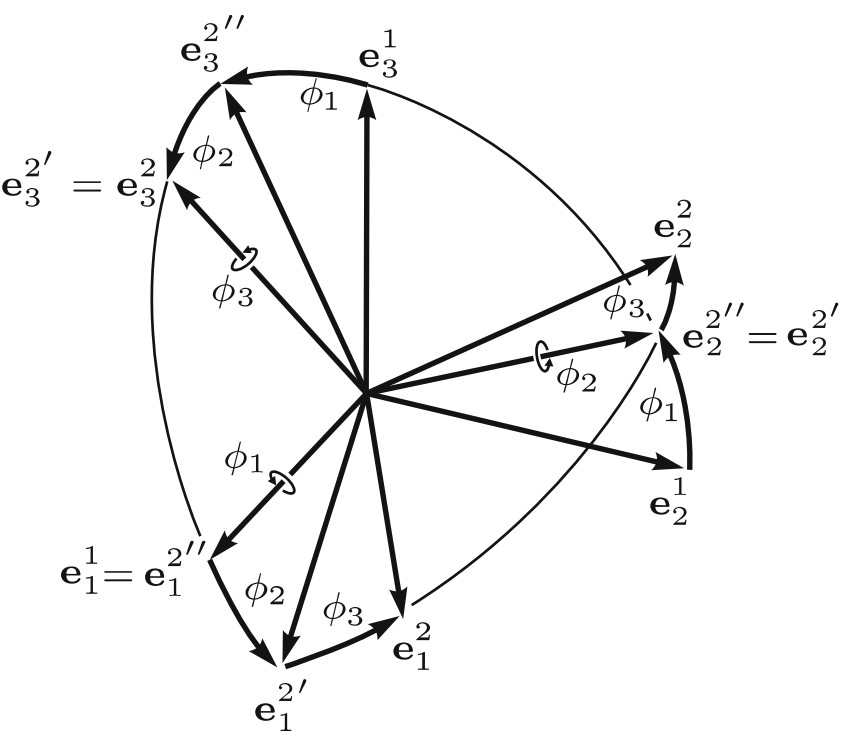
\includegraphics[width=5cm]{bryanangles}
			\caption{representation of the Bryan angles $\phi_1,\phi_2,\phi_3$ for representing the attitude of a body.}
		\end{SCfigure}
	
		\paragraph{Inverse sequence} Until now we considered the \textbf{direct sequence} in order to describe the attitude of a local reference frame $\bb$ respect to the global base $\bw$, but sometime the inverse operation is required (to describe the attitude of a vector in $\bb$ knowing it's coordinates in $\bw$). In this case we have that the \textbf{inverse sequence} of rotation is obtained by inverting the rotation sequence and changing the sign to the angles as in this example:
		\begin{equation} \label{eq:rot:inversesequence}
			\textrm{direct seq.: } \R = \R_z(\psi) \R_x(\phi)\R_y(\theta) \qquad \mapsto \qquad \textrm{inverse seq.: } \R^{-1} = \R_y(-\theta) \R_x(-\phi) \R_z(-\psi)
		\end{equation}
	
		\paragraph{Singular configuration} In general the same orientation of the body can be expressed as function of different angles depending on the rotation sequence chosen, but however anyone of this representation presents a \de{singular configuration} (also referred s the \textbf{\textit{gimbal lock}}) where for particular values of the intermediate rotation this description doesn't allow to fully discriminate the attitude of the body. Considering as example the Euler angle representation (equation \ref{eq:kin:eulerangles}) in case of $\theta = k\pi$ (where $k\in \mathds Z$), the evaluation and subsequence simplification of the matrix results in
		\[ \R_z(\phi) \R_x(0) \R_z(\psi) = \matrix{ \cos(\phi + \psi) & \sin(\phi + \psi) & 0 \\ -\sin(\phi+\psi) & \cos(\phi+\psi) & 0 \\ 0 & 0 & 1 } \]
		As we can see such sequence results in a rotation matrix along the $z$ axis of the starting reference frame of an angle $\phi+\psi$, hence we have only one parameter (instead of the required 3) to describe the orientation of the body, hence we have 2 degree of freedom left unknown.
		
		\paragraph{From rotation matrix to angles} In general problems what we might have is a rotation matrix $\R$ (whose components are described in equation \ref{eq:rot:rotationmatrix}) with 9 entries subjected to 6 constraints but that we want are a sequence of primitive rotations hence their associated angles. This operation can be obtained by solving the non-linear systems associated to $\R_i(\phi) \R_j(\theta) \R_k(\psi) = \R$ (where $i,j,k$ are generically axis of rotation); such operation should be performed on the 3 \textit{easier} expression. Considering as example the sequence of rotation $z(\psi) \rightarrow y(\theta) \rightarrow x (\phi)$ what we obtain is the equality
		\[ \matrix{\cos \theta \cos\psi & -\cos\theta \sin \psi & \sin\psi \\
		\sin\phi\sin\theta\cos\psi + \cos\phi \sin\psi & -\sin\phi\sin\theta\sin\psi + \cos\phi\cos\psi & -  \sin\phi\cos\theta \\
		-\cos\phi \sin\theta\cos\psi + \sin\phi\sin\psi & \cos\phi \sin\theta\sin\psi + \sin\phi\cos\psi & \cos\phi\cos\theta  } = \matrix{ u_x  &  v_x & w_x \\ u_y  &  v_y & w_y \\ u_z  &  v_z & w_z } \]
		The easier terms to match are $\cos\theta \cos\phi = u_x$, $-\cos\theta\sin \psi = v_x$ and $-\sin\phi\cos\theta = w_y$ that, simultaneously solved, determines the angles
		\begin{equation}
		\begin{split}
			\phi & = \arctan\left( - \frac{u_x}{\sqrt{u_x^2+w_y^2}}, \frac{w_y}{\sqrt{u_x^2 + w_y^2}} \right) \hspace{2cm} \theta = -\arccos\left( - \sqrt{u_x^2 + w_y^2} \right) \\			
			\psi &= \pi - \arcsin \left(\frac{v_x}{\sqrt{u_x^2 + w_y^2}}\right)
		\end{split}
		\end{equation}
		In reality this is just one of the multiple solutions of the non-linear system (in this particular case symbolic solvers determine 8 different solutions for the angles that satisfy the 3 equation) hence multiple combination of angles $\phi,\theta,\psi$ can lead to the same rotation matrix.
		
	\subsection{Rotation axis, Euler theorem and quaternions}
		As was previously stated, the rotation matrix $\R$ relates the relative orientation of two bases $\base 1,\base 2$; being that such matrix lies in the set of the special orthogonal matrices is characterised by having the inverse equal to the transpose and has $\det \R=1$. Another important property that can be obtained is by considering the \textbf{eigenvalue problem} $\R \vett v_b = \lambda \vett v_w$, meaning that we would like to find if there's a vector $\vett v$ whose orientation isn't altered after the transformation has occurred. Mathematically to compute such problem we have to first compute the eigenvalues as
		\[ \det\big(\R - \lambda \I\big) = p(\lambda) = 0 \]
		where $p(\lambda)$ is the characteristic polynomial of $\R$ that evaluates to
		\begin{align*}
			p(\lambda) & = - \lambda^3 + \lambda^2 \trace{\R} - \lambda \trace{\R} + \det \R \\
			& = (\lambda - 1) \left( \lambda^2 - (\trace \R - 1) \lambda + 1 \right)  
		\end{align*}
		It is also proven (as shown) that such characteristic polynomial has always a unitary eigenvalue, meaning that always exists one direction of transformation that remain unaltered in both \textit{orientation} and \textit{elongation}: this direction is hence called \de{rotation axis}. Moreover the other two eigenvalues $\lambda_{2,3}$ of $p(\lambda)$ are complex conjugated and are used to determine the \de{rotation angle} $\varphi$ of the transformation along the rotation axis:
		\[ \lambda_{2,3} = \frac{\trace{\R} -1 }{2} \pm j \sqrt{1- \left( \frac{\trace \R - 1}{2} \right)^2} = \cos\varphi \pm j \sin\varphi = e^{\pm j\varphi} \]
		\begin{equation}
			\Rightarrow \qquad  \varphi = \arccos\left( \frac{\trace \R - 1}{2} \right)
		\end{equation}
		
		Note that the eigensystem doesn't result in one unique solution: if we denote $\R(\vers n,\theta)$ the rotation of an angle $\theta$ along the direction $\vers n$, then the same transformation can be obtained considering the opposite axis and angle:
		\[ \R(-\vers n ,-\theta) = \R(\vers n,\theta) \]
		This way of defining rotations is also periodic, in the sense that we can restrict any transformation along on axis to an angle $\theta\in[0,2\pi]$
		\[ \R(\vers n,\theta + 2k\pi) = \R(\vers n,\theta) \qquad \forall k \in \mathds Z \]
		Moreover if we consider a rotation with rotation angle $\theta=0$, then such transformation is undetermined (in fact no displacement occurs). With all this premises the \de{Euler theorem} holds and states that {\itshape the displacement of a body-fixed base from an initial position $\base^1$ to an arbitrary final position $\base^2$ is achieved by a rotation through a certain angle about an axis which is fixed in both bases. The axis has the direction of the eigenvector associated with the eigenvalue $\lambda= 1$ of the direction cosine matrix $\R$. }
		
		\paragraph{Rotation matrix given an axis and the angle} In practical application we might want to have that a rotation of an angle $\theta$ occurs along a certain direction $\vers n$; in order so to compute the rotation matrix $\R(\vers n, \theta)$, a way to do so is to firstly apply two generic rotation (as example $\R_z(\alpha) \R_x(\beta)$) in order to have a reference frame $\rf{temp}$ whose third base component $\vers k_{temp}$ is aligned with the direction $\vers n$ in the ground reference frame. On such frame we can compute the rotation of the angle $\theta$ (along the $z$ axis) but in order to obtain the final reference frame we have to apply the inverse transformation $\rf{temp}^{-1} = \R_x(-\alpha) \R_z(-\beta)$ (using the result of equation \ref{eq:rot:inversesequence}). The rotation matrix can so be regarded as
		\begin{equation}
			\R(\vers n,\theta) = \R_x(\alpha) \R_y(\beta) \R_z(\theta) \R_y(-\beta) \R_x(-\alpha)
		\end{equation}
		At this point all that's left is to determine such angles $\alpha,\beta$ in order to have the alignment of the temporary reference frame with the chosen direction $\vers n$: considering that the associated rotation matrix is
		\[ \R(\alpha,\beta) = \R_x(\alpha) \R_y(\beta) = \matrix{\vers i_2(\alpha,\beta) | \vers j_2(\alpha,\beta) | \vers k_2(\alpha,\beta)} \]
		where $\vers i_2,\vers j_2,\vers k_2$ are the versor of the temporary base $\base^{temp}$ in global coordinates and so in order to have that $\vers k_2$ is parallel to $\vers n$ we have to solve the non-linear system in $\alpha,\beta$ determined as
		\[ \begin{cases}
			\vers n \cdot \vers i_2 = 0 \\ \vers n\cdot \vers j_2 = 0
		\end{cases} \]
	
		\paragraph{Rodrigues formula} Given a rotation axis $\vers n$ and the rotation angle $\theta$, the \de{Rodrigues formula} allows to compute the rotated coordinates $\vett r_w^{rot}$ of a vector with starting components $\vett r_b$:
		\begin{equation}
			\vett r_w^{rot} = \cos\theta \, \vett r_b + (1-\cos\theta) (\vers n \cdot \vett r_b) \vers n + \sin\theta \, \vers n\times \vett r_b 
		\end{equation}
		Considering that $(\vers n \cdot \vett r_b) \vers n$ can be regarded as $\vett r_v + \vers n \times (\vers n\times \vers r_b)$ but also that the vectorial product $\vers n \times \vett v$ (with $\vett v \in \mathds R^3$ is a generic vector) can be regarded as the following matrix product
		\begin{equation}
			\mat N_s \vett v := \matrix{ 0 & - n_z & n_y \\ n_z & 0 & -n_x \\ -n_y & n_x & 0} \vector{v_x \\ v_y \\ v_z}
		\end{equation}
		With this we can rewrite Rodrigues formula as
		\begin{equation}
			\vett r_w^{rot} = \Big( I + (1-\cos\theta) \mat N_s \mat N_s + \sin\theta \mat N_s \Big) \vett r_b 
		\end{equation}
		
		\begin{note}
			In general any vectorial product $\vett w \times \vett v$ can be reduced to a matrix multiplication in the form $\mat W \vett v$, where $\mat W \in \mathds R^{3\times 3}$ is a skew-symmetric matrix in the form shown. 
		\end{note}
	
		By defining $q_0 = \cos(\theta/2)$ and $\tilde{\vett q} = (q_1,q_2,q_3) = \vers n \sin(\theta/2) = \big(n_x \sin(\theta/2), n_y\sin(\theta/2), n_z\sin(\theta/2)\big)$ what we obtain are the 4 \de{Euler-Rodrigues parameters}; in particular $\tilde{\vett q}$ is a vector lying in the rotation axis (is in fact proportional by a factor $\sin(\theta/2)$ to $\vers n$). Such formulation is characterized by having that
		\[ \sum_{i=0}^3 q_i^2 = 1 \]
		The vector $\vett q = (q_0,\tilde{\vett q}) = (q_0, q_1, q_2, q_3) \in \mathds R^4$ is the so called \de{quaternion} and allows to give a global parametrization of the rotation matrix $\R$ (it is said \textit{global} because it doesn't require the definition of intermediate reference frames to determine the rotations). We can in fact show that each rotation matrix can be expressed in quaternions as
		\begin{equation} \label{eq:rot:quaternionmatrix}
			\R(\vett q) = \matrix{ 2q_0^2 + 2 q_1^2 - 1 & - 2q_0 q_3 + 2q_1 q_2 & 2q_0 q_2 + 2q_1 q_3 \\ 2 q_0 q_3 + 2 q_1 q_2 & 2q_0^2 + 2 q_2^2 - 1 & - 2 q_0 q_1 + 2 q_2 q_3 \\ -2q_0q_2 +2 q_1 q_3 & 2 q_0 q_1 +2 q_2q_3 & - 2 q_1^2 -2 q_2^2+1 }
		\end{equation}
		Such parametrization has 4 parameters, but only 3 of them are independent and so, while describing systems in such representation, the following constraint equation must always be introduced:
		\[ q_0^2 + q_1^2 + q_2^2 + q_3^2 = 1 \]
		The cost of adding one more parameter in the description of the system (and the related constraint equation) comes with the advantage of having a representation that's always non-singular (so it doesn't have the gimbal lock problem, as for \textit{common} rotation sequences that are intuitively easier to understand and physically interpret). 
		
		\textbf{CHIEDERE LA CONFIGURAZIONE SINGOLARE PER $\theta = 0$ o $q_0 = 0$?x}
		
	\subsection{Velocities and acceleration}
		Usually reference frames moves respect to each other, and so in general is important to understand how velocities (and accelerations) in local frames relates to their respective in global coordinates. For this reason we determine the \de{angular rate} $\vett \omega = (\omega_x,\omega_y,\omega_z)$ as the vector of 3 components that represents the rate of change of a reference frame with respect to another one (typically the world reference frame).
		
		Given a vectorial base characterized by the rotation matrix $\R$, compute the derivative of it's components in time $t$ determines the rate of change $\dot \R$ of the body in the world reference frame. Considering that $\R^T = \R^{-1}$ is  the inverse rotation matrix that match the world coordinates with the body one, we have that
		\begin{equation}
			\R^T \dot \R = \matrix{0 & - \omega_z & \omega_y \\ \omega_z & 0 & - \omega_x \\ -\omega_y & \omega_x & 0} = \Po
		\end{equation}
		where $\Po$ is a skew-symmetric matrix usual referred as \de{angular operator} that's used to implement the vectorial product of $\vett \omega$: it happens that $\vett \omega \times \vett x = \Po \vett x$ for any vector $\vett x \in \mathds R^3$. In particular $\vett \omega$ represent the projection of the rotation axis in the local reference frame; moreover if we consider $\vett u \in \mathds R^m$ the vector of the parameters used in the description of the attitude of the body, the angular rate can be regarded as a linear combination of the rate of changes of such parameters:
		\[ \vett \omega^b = \vector{\omega_x \\ \omega_y \\ \omega_z} = \mat E(\vett u) \, \dvett u \qquad \mat E(\vett u) \in \mathds R^{n\times m}\]
		In particular
		\begin{itemize}
			\item if we consider a set of 3 independent parameters as the 3 angles $\vett u = (\alpha,\beta,\theta)$ generating the rotation matrix $\R= \R_x(\alpha) \R_y(\beta) \R_z(\theta)$ we can compute the angular operator $\Po = \mat R^T \dot{\mat R}$ determining 
			\[ \vett \omega^b = \underbrace{ \matrix{ \sin \beta & 0 & 1 \\ \cos\beta\sin\theta & \cos\theta & 0 \\ \cos\beta \cos\theta & \sin\beta & 0 }}_{=\mat E(\vett u)} \underbrace{\vector{\dot \alpha \\ \dot \beta \\ \dot \theta}}_{=\dvett u} \]
			\item if we would have instead a quaternion representation $\vett u = (q_0,q_1,q_2,q_3)$, considering the definition in equation \ref{eq:rot:quaternionmatrix} for the rotation matrix, from the computation $\R^T \dot \R = \Po$ we would have obtained
			\[ \vett \omega^b = 2 \matrix{ q_3 & q_2 & - q_1 & q_0 \\ q_2 & - q_1 & - q_0 & q_3 \\ -q_1 & q_0 & q_3 & q_2 } \vector{\dot q_0 \\ \dot q_1 \\ \dot q_2 \\ \dot q_3} \]
			The number of free parameters is 3 because one is constrained by the equation $q_0^2 + q_1^2 + q_2^2 + q_3^2 = 1$ and so, also in this case, we have to consider the differential of such constraint in order to univocally determine the angular velocity:
			\[ \frac{d}{dt} \big(\vett q \cdot \vett q = 1 \big) \qquad \rightarrow \qquad 2q_0 \dot q_0 + 2 q_1 \dot q_1 + 2q_2\dot q_2 + 2 q_3 \dot q_3 = 0 \]
		\end{itemize}
		We observe so that the problem of the velocities is linear if we know the actual configuration/position of the system.
		
		
		\paragraph{Velocity} Recalling equation \ref{eq:rot:directtransformation}, the global coordinates $\vett P^w$ of a point described by $\vett P^b$ in a local reference frame is defined as
		\[ \vett P^w = \vett P_0 + \R \vett P^b \]
		where $\vett P_0$ is the origin of the moving frame in the global coordinates. Differentiating in time allows to determine the velocity
		\begin{equation} \label{eq:rot:velocity}
		\begin{split}
			(\ref{eq:rot:directtransformation}) \qquad \xrightarrow{\frac d{dt}} \qquad \dvett P^w & = \dvett P_0 + \dot \R \vett P^b + \R \dvett P^b = \dvett P_0 + \overbrace{\R \R^T}^{=\I} \R \vett P^b + \R \dvett P^b \\
			& = \dvett P_0 + \R \Po \vett P^b + \R \dvett P^b
		\end{split}
		\end{equation}
		where $\dvett P_0$ is the contribution due to the velocity in the translation of the local frame, $\R \Po \vett P^b$ is due to the frame angular velocity and $\R \dvett P^b$ is an optional terms that considers the relative velocity $\dvett P^b$ that the point might have in the local frame. The associated \textbf{transformation matrix} is so
		\[ \dvett P^w = \matrix{ \begin{array}{c|c}
			\R\Po & \dvett P_0 \\ \hline \vett 0^t & 0 
		\end{array}} \vett P^b + \matrix{ \begin{array}{c|c}
			\R & \dvett P_0 \\ \hline \vett 0^t & 1 
		\end{array}} \dvett P^b\]
	
		\paragraph{Acceleration} Differentiating \ref{eq:rot:velocity} one more time respect to time allows to compute the \textbf{acceleration} of the point $P$ in the global reference frame as
		\[ (\ref{eq:rot:velocity}) \qquad \xrightarrow{\frac d{dt}} \qquad \ddvett P^w = \ddvett P_0 + \ddot\R \vett P^b + \dot \R \dvett P^b + \dot \R \dvett P^b + \R \ddvett P^b \]
		Considering that $ \ddot \R = \frac d{dt} \dot \R= \frac d{dt} \left(\R \Po\right) = \dot \R \Po + \R \dPo = \R \R^T \dot \R \Po + \R \Po \Po$ what we obtain is
		\begin{equation}
			\begin{split}
				\ddvett P^w & = \ddvett P_0 + \R \Po\Po \vett P^b + \R \dPo \vett P^b + 2 \R \Po \dvett P_b + \R \ddvett P^b \\ 
				& = \ddvett P_0 + \R \underbrace{\Big( \underbrace{\Po \Po \vett P^b}_\textrm{centripetal acc.} + \underbrace{\dPo \vett P^b}_\textrm{tangential acc.} + \underbrace{2 \Po \dvett P^b + \ddvett P^b}_\textrm{relative acc} \Big)}_\textrm{acceleration in the local frame}
			\end{split}
		\end{equation}
	
	\subsection{Natural coordinates}
		In general rotation matrices $\R$ can be expressed with any set of parameters we want; the idea is that the matrix $\R = \matrix{i_x & j_x & k_x \\ i_y & j_y & k_y \\ i_z & j_z & k_z }$ can be described with 9 parametric components constrained by 6 equation: this determines a more redundant formulation that however generates a new way to describe the configuration of bodies. The main idea is now to use global coordinates of points (that mechanically can be associated to joints) or vector (that can represent the direction relative translation/rotation of two elements) in order to build the rotation matrix $\R$.
		
		The advantage of this approach is that we have at maximum quadratic equations that can easily solved numerically by calculators with the problem that quadratic constraints generates 2 solutions each.
		
		\paragraph{Planar case with two points} If we consider two points $P_1,P_2$ lying in the same rigid body (hence their distance $L$ is fixed) characterized by global cartesian coordinates $(x_1,y_1),(x_2,y_2)$ respectively (for simplicity we consider a planar case), the whole system can be described with the coordinates $\vett q = (x_1, y_1, x_2, y_2)$. In order to determine $\R$ (that requires 3 independent parameters) as function of $\vett q$ (that actually has 4 parameters) we need to determine one constraint equation.
		
		In order to determine the moving reference frame it is necessary firstly to chose one point as origin of such frame (in this case we consider $P_1$) and we have to orient one versor of the frame (in this case $\vers i_1$) with the vector $\vett P_1 \vett P_2$ connecting the two points. Being the body rigid we have that the constraint equation is related to the length between the points that's fixed, in fact
		\[ \vett P_1\vett P_2 \cdot \vett P_1\vett P_2 = L^2 \]
		By what we just stated, the first versor $\vers i_1$ of the moving frame in global coordinates can be computed as the normalization of the vector $\vett P_1\vett P_2$, hence
		\[ \vers i_1 = \frac{\vett P_1 \vett P_2}{L} = \vector{ \frac{x_2- x_1}{L} \\ \frac{y_2 - y_1}{L} \\ 0} = \vector{i_{1x} \\ i_{1y} \\ i_{1z} } \]
		The goal now is to determine the coordinates of the other versor $\vers j_1$ that compose the rotation matrix that, in the planar case, has the form
		\[ \R = \matrix {i_{1x} & j_{1x} & 0 \\ i_{1y} & j_{1y} & 0 \\ 0 & 0 & 1 }  \]
		Knowing that a proper rotation matrix requires $\vers i_1 \cdot \vers j_1 = 0$ we obtain the relation
		\[ i_{1x}j_{1x} + i_{1y} j_{1y} = 0 \qquad \Rightarrow \qquad j_{1x} = - \frac{i_{1y}}{i_{1x}} j_{1y} = - \frac{y_2 - y_1}{x_2-x_1} j_{1y} \]
		Knowing that it must also hold $\vers j_1 \cdot \vers j_1 = 1$ we build the quadratic relation
		\[ j_{1x}^2 + j_{1y}^2 = j_{1y}^2\left( 1 + \frac{(y_2-y_1)^2}{ (x_2 - x_1)^2 } \right) = 1 \qquad \Rightarrow \qquad \Rightarrow j_{1y} = \pm \frac{x_2-x_1}{L} \]
		We so have that the 2 possible formulation of the rotation matrix are
		\[ \R = \matrix { \frac{x_2 - x_1}{L} & -\frac{y_2 - y_1}{L} & 0 \\ \frac{y_2 - y_1}{L} & \frac{x_2 - x_1}{L} & 0 \\ 0 & 0 & 1 } \qquad \textrm{or} \qquad \R = \matrix { \frac{x_2 - x_1}{L} & \frac{y_2 - y_1}{L} & 0 \\ \frac{y_2 - y_1}{L} & - \frac{x_2 - x_1}{L} & 0 \\ 0 & 0 & 1 }  \]
		that are subjected to
		\[ (x_2-x_1)^2 + (y_2 - y_1)^2 = L^2 \]
		The problem of this formulation is that it isn't intuitive the rotation $\alpha$ of the reference frame respect to the global direction $\vers i_0$, however this can be achieved equating $\R$ with the rotation matrix function of $\alpha$:
		\[ \matrix { \frac{x_2 - x_1}{L} & -\frac{y_2 - y_1}{L} & 0 \\ \frac{y_2 - y_1}{L} & \frac{x_2 - x_1}{L} & 0 \\ 0 & 0 & 1 } = \matrix { \cos\alpha & - \sin \alpha & 0 \\ \sin\alpha & \cos \alpha & 0 \\ 0 & 0 & 1} \quad \Rightarrow \quad \sin\alpha = \frac{y_2 - y_1}{2} \quad \Rightarrow \quad \alpha = \arcsin \left( \frac{y_2 - y_1}{2} \right)  \]
		
		
		
		
		
		
		
		
		
		
		
		
		
		
		
		
		
		
		
		
		
		
		
		
		
		
		
		
		
		
		
		
		
		
		
		